\documentclass{article}\usepackage[]{graphicx}\usepackage[]{xcolor}
% maxwidth is the original width if it is less than linewidth
% otherwise use linewidth (to make sure the graphics do not exceed the margin)
\makeatletter
\def\maxwidth{ %
  \ifdim\Gin@nat@width>\linewidth
    \linewidth
  \else
    \Gin@nat@width
  \fi
}
\makeatother

\definecolor{fgcolor}{rgb}{0.345, 0.345, 0.345}
\newcommand{\hlnum}[1]{\textcolor[rgb]{0.686,0.059,0.569}{#1}}%
\newcommand{\hlsng}[1]{\textcolor[rgb]{0.192,0.494,0.8}{#1}}%
\newcommand{\hlcom}[1]{\textcolor[rgb]{0.678,0.584,0.686}{\textit{#1}}}%
\newcommand{\hlopt}[1]{\textcolor[rgb]{0,0,0}{#1}}%
\newcommand{\hldef}[1]{\textcolor[rgb]{0.345,0.345,0.345}{#1}}%
\newcommand{\hlkwa}[1]{\textcolor[rgb]{0.161,0.373,0.58}{\textbf{#1}}}%
\newcommand{\hlkwb}[1]{\textcolor[rgb]{0.69,0.353,0.396}{#1}}%
\newcommand{\hlkwc}[1]{\textcolor[rgb]{0.333,0.667,0.333}{#1}}%
\newcommand{\hlkwd}[1]{\textcolor[rgb]{0.737,0.353,0.396}{\textbf{#1}}}%
\let\hlipl\hlkwb

\usepackage{framed}
\makeatletter
\newenvironment{kframe}{%
 \def\at@end@of@kframe{}%
 \ifinner\ifhmode%
  \def\at@end@of@kframe{\end{minipage}}%
  \begin{minipage}{\columnwidth}%
 \fi\fi%
 \def\FrameCommand##1{\hskip\@totalleftmargin \hskip-\fboxsep
 \colorbox{shadecolor}{##1}\hskip-\fboxsep
     % There is no \\@totalrightmargin, so:
     \hskip-\linewidth \hskip-\@totalleftmargin \hskip\columnwidth}%
 \MakeFramed {\advance\hsize-\width
   \@totalleftmargin\z@ \linewidth\hsize
   \@setminipage}}%
 {\par\unskip\endMakeFramed%
 \at@end@of@kframe}
\makeatother

\definecolor{shadecolor}{rgb}{.97, .97, .97}
\definecolor{messagecolor}{rgb}{0, 0, 0}
\definecolor{warningcolor}{rgb}{1, 0, 1}
\definecolor{errorcolor}{rgb}{1, 0, 0}
\newenvironment{knitrout}{}{} % an empty environment to be redefined in TeX

\usepackage{alltt}
\usepackage[margin=1.0in]{geometry} % To set margins
\usepackage{amsmath}  % This allows me to use the align functionality.
                      % If you find yourself trying to replicate
                      % something you found online, ensure you're
                      % loading the necessary packages!
\usepackage{amsfonts} % Math font
\usepackage{fancyvrb}
\usepackage{hyperref} % For including hyperlinks
\usepackage[shortlabels]{enumitem}% For enumerated lists with labels specified
                                  % We had to run tlmgr_install("enumitem") in R
\usepackage{float}    % For telling R where to put a table/figure
\usepackage{natbib}        %For the bibliography
\bibliographystyle{apalike}%For the bibliography
\IfFileExists{upquote.sty}{\usepackage{upquote}}{}
\begin{document}


\begin{enumerate}
%%%%%%%%%%%%%%%%%%%%%%%%%%%%%%%%%%%%%%%%%%%%%%%%%%%%%%%%%%%%%%%%%%%%%%%%%%%%%%%%
%%%%%%%%%%%%%%%%%%%%%%%%%%%%%%%%%%%%%%%%%%%%%%%%%%%%%%%%%%%%%%%%%%%%%%%%%%%%%%%%
% Question 1
%%%%%%%%%%%%%%%%%%%%%%%%%%%%%%%%%%%%%%%%%%%%%%%%%%%%%%%%%%%%%%%%%%%%%%%%%%%%%%%%
%%%%%%%%%%%%%%%%%%%%%%%%%%%%%%%%%%%%%%%%%%%%%%%%%%%%%%%%%%%%%%%%%%%%%%%%%%%%%%%%
\item When conducting the work of Lab 11, we conducted the test that uses the
Central Limit Theorem even though the sample size was ``small" (i.e., $n<30$).
It turns out, that how ``far off" the $t$-test is can be computed using
a first-order Edgeworth approximation for the error. Below, we will do this 
for the the further observations.
\begin{enumerate}
  \item \cite{Boos00} note that 
  \begin{align*}
    P(T \leq t) \approx F_Z(t) + \underbrace{\frac{\text{skew}}{\sqrt{n}} \frac{(2t^2+1)}{6} f_Z(t)}_{\textrm{error}},
  \end{align*}
  where $f_Z(\cdot)$ and $F_Z(\cdot)$ are the Gaussian PDF and CDF and skew is the
  skewness of the data. What is the potential error in the computation of the 
  $p$-value when testing $H_0: \mu_X=0; H_a: \mu_X<0$ using the zebra finch further data? 
  
\begin{knitrout}\scriptsize
\definecolor{shadecolor}{rgb}{0.969, 0.969, 0.969}\color{fgcolor}\begin{kframe}
\begin{alltt}
\hlkwd{library}\hldef{(tidyverse)}
\hlkwd{library}\hldef{(xtable)}
\hlkwd{library}\hldef{(e1071)}
\hlcom{###############################################################################}
\hlcom{# Question 1}
\hlcom{###############################################################################}

\hlcom{# part a}
\hldef{zebra} \hlkwb{<-} \hlkwd{read.csv}\hldef{(}\hlsng{"zebrafinches.csv"}\hldef{)}

\hldef{further} \hlkwb{<-} \hldef{zebra}\hlopt{$}\hldef{further}
\hldef{n} \hlkwb{<-} \hlkwd{length}\hldef{(further)}
\hldef{skew} \hlkwb{<-} \hlkwd{skewness}\hldef{(further)}

\hlcom{# t test\}}
\hldef{t_result} \hlkwb{<-} \hlkwd{t.test}\hldef{(further,} \hlkwc{mu}\hldef{=}\hlnum{0}\hldef{,} \hlkwc{alternative}\hldef{=}\hlsng{"less"}\hldef{)}
\hldef{t_stat} \hlkwb{<-} \hldef{t_result}\hlopt{$}\hldef{statistic}

\hlcom{# Gaussian PDF and CDF}
\hldef{fz} \hlkwb{<-} \hlkwd{dnorm}\hldef{(t_stat)}
\hldef{Fz} \hlkwb{<-} \hlkwd{pnorm}\hldef{(t_stat)}

\hlcom{# Edgeworth error approx}
\hldef{(error} \hlkwb{<-} \hldef{(skew} \hlopt{/} \hlkwd{sqrt}\hldef{(n))} \hlopt{*} \hldef{((}\hlnum{2}\hlopt{*}\hldef{t_stat}\hlopt{^}\hlnum{2} \hlopt{+} \hlnum{1}\hldef{)} \hlopt{/} \hlnum{6}\hldef{)} \hlopt{*} \hldef{fz)}
\end{alltt}
\begin{verbatim}
##             t 
## -1.226006e-13
\end{verbatim}
\begin{alltt}
\hldef{(probability} \hlkwb{<-} \hldef{Fz} \hlopt{+} \hldef{error)}
\end{alltt}
\begin{verbatim}
##             t 
## -1.189164e-13
\end{verbatim}
\end{kframe}
\end{knitrout}

Using the Edgeworth approximation, we calculated the error in the \emph{p}-value when
applying the Central Limit Theorem despite a small sample size. 
For the further data, we computed the sample skewness and used it along with the observed
\emph{t}-statistic from a one-sided \emph{t}-test. The resulting approximation yielded
an error of $-1.23 * 10^{-13}$, meaning the true p-value differs from the normal
approximation by an extremely small amount. This is because the \emph{t}-statistic
lies far in the tail, where the normal and true distributions closely align. The 
adjusted probability, incorporating the correction, is essentially the same as
the unadjusted one: $-1.19 * 10^{-13}$

  \item Compute the error for $t$ statistics from -10 to 10 and plot a line
  that shows the error across $t$. Continue to use the skewness and 
  the sample size for the zebra finch further data.
  
\begin{knitrout}\scriptsize
\definecolor{shadecolor}{rgb}{0.969, 0.969, 0.969}\color{fgcolor}\begin{kframe}
\begin{alltt}
\hlcom{# part b}
\hldef{t_vals} \hlkwb{<-} \hlkwd{seq}\hldef{(}\hlopt{-}\hlnum{10}\hldef{,} \hlnum{10}\hldef{,} \hlkwc{by}\hldef{=}\hlnum{0.1}\hldef{)}
\hldef{fz_vals} \hlkwb{<-} \hlkwd{dnorm}\hldef{(t_vals)}
\hldef{error_vals} \hlkwb{<-} \hldef{(skew} \hlopt{/} \hlkwd{sqrt}\hldef{(n))} \hlopt{*} \hldef{((}\hlnum{2}\hlopt{*}\hldef{t_vals}\hlopt{^}\hlnum{2} \hlopt{+} \hlnum{1}\hldef{)} \hlopt{/} \hlnum{6}\hldef{)} \hlopt{*} \hldef{fz_vals}

\hldef{error_df} \hlkwb{<-} \hlkwd{data.frame}\hldef{(}\hlkwc{t}\hldef{=t_vals,} \hlkwc{error}\hldef{=error_vals)}

\hlkwd{ggplot}\hldef{(}\hlkwc{data} \hldef{= error_df,} \hlkwd{aes}\hldef{(}\hlkwc{x}\hldef{=t,} \hlkwc{y}\hldef{=error))} \hlopt{+}
  \hlkwd{geom_line}\hldef{(}\hlkwc{color}\hldef{=}\hlsng{"red"}\hldef{,} \hlkwc{linewidth}\hldef{=}\hlnum{1}\hldef{)} \hlopt{+}
  \hlkwd{xlab}\hldef{(}\hlsng{"T-Statistic"}\hldef{)} \hlopt{+}
  \hlkwd{ylab}\hldef{(}\hlsng{"Error"}\hldef{)} \hlopt{+}
  \hlkwd{ggtitle}\hldef{(}\hlsng{"First-Order Edgeworth Approximation for Error"}\hldef{)} \hlopt{+}
  \hlkwd{theme_bw}\hldef{()}
\end{alltt}
\end{kframe}
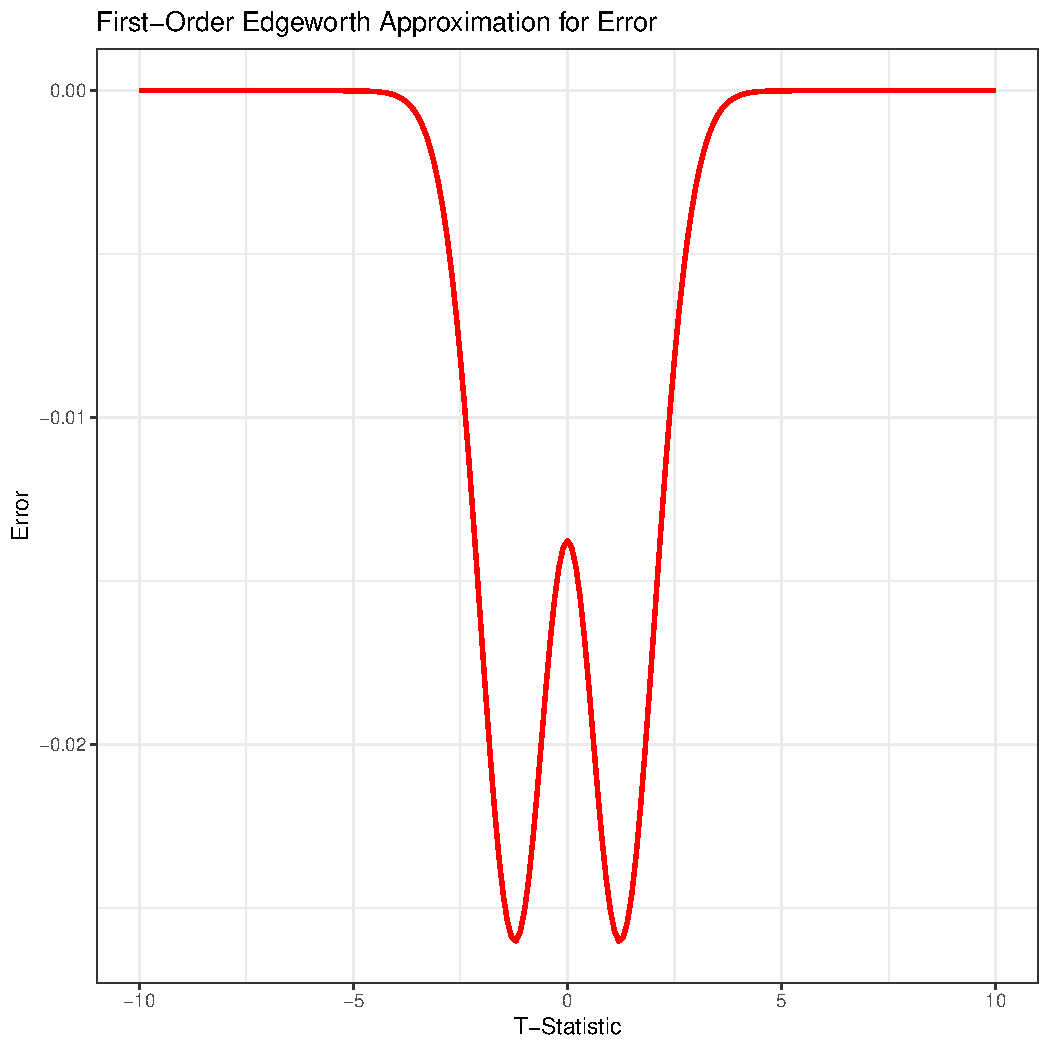
\includegraphics[width=\maxwidth]{figure/unnamed-chunk-3-1} 
\end{knitrout}



To understand how this error behaves across different \emph{t}-values, we computed the 
approximation over a range from -10 to 10. The resulting plot shows how the error
varies as a function of the \emph{t}-statistic. The plot takes on a ``W" shape, with
the error approaching zero in the extreme tails.This occurs because, when the 
\emph{t}-statistic is very large or small, the cumulative probability under the
normal curve is already close to 0 or 1. In these regions, small corrections due
to skewness have little effect. In contrast, around the boundaries of typical
rejection regions, the cumulative probability is more sensitive to such shifts,
leading to larger errors. This visualization highlights how skewness primarily
distorts inference in the moderate \emph{t}-range rather than the extremes.


  \item Suppose we wanted to have a tail probability within 10\% of the desired
  $\alpha=0.05$. Recall we did a left-tailed test using the further data.
  How large of a sample size would we need? That is, we need
  to solve the error formula equal to 10\% of the desired left-tail probability:
  \[0.10 \alpha  \stackrel{set}{=} \underbrace{\frac{\text{skew}}{\sqrt{n}} \frac{(2t^2+1)}{6} f_Z(t)}_{\textrm{error}},\]
  which yields
  \[ n = \left(\frac{\text{skew}}{6(0.10\alpha)} (2t^2 + 1) f_Z(t)\right)^2.\]
  
Finally, we used the Edgeworth approximation to determine how large the sample
size must be to ensure that the tail probability under the normal approximation
is within 10\% of the nominal $\alpha = 0.05$. We found that approximately
521 observations are required. This large sample size reflects the impact of 
skewness on inference: when the data are skewed, much larger samples are needed
to trust results based on the normal approximation- especially for accurate inference
in the tails of the distribution.
  
\end{enumerate}
%%%%%%%%%%%%%%%%%%%%%%%%%%%%%%%%%%%%%%%%%%%%%%%%%%%%%%%%%%%%%%%%%%%%%%%%%%%%%%%%
%%%%%%%%%%%%%%%%%%%%%%%%%%%%%%%%%%%%%%%%%%%%%%%%%%%%%%%%%%%%%%%%%%%%%%%%%%%%%%%%
% Question 2
%%%%%%%%%%%%%%%%%%%%%%%%%%%%%%%%%%%%%%%%%%%%%%%%%%%%%%%%%%%%%%%%%%%%%%%%%%%%%%%%
%%%%%%%%%%%%%%%%%%%%%%%%%%%%%%%%%%%%%%%%%%%%%%%%%%%%%%%%%%%%%%%%%%%%%%%%%%%%%%%%
\item Complete the following steps to revisit the analyses from lab 11 using the
bootstrap procedure.
\begin{enumerate}
\item Now, consider the zebra finch data. We do not know the generating distributions
for the closer, further, and difference data, so perform resampling to approximate the 
sampling distribution of the $T$ statistic:
  \[T = \frac{\bar{x}_r - 0}{s/\sqrt{n}},\]
  where $\bar{x}_r$ is the mean computed on the r$^{th}$ resample and $s$ is the
  sample standard deviation from the original samples. At the end, create an
  object called \texttt{resamples.null.closer}, for example, and store the 
  resamples shifted to ensure they are consistent with the null hypotheses at the average 
  (i.e., here ensure the shifted resamples are 0 on average, corresponding
  to $t=0$, for each case). 

\begin{knitrout}\scriptsize
\definecolor{shadecolor}{rgb}{0.969, 0.969, 0.969}\color{fgcolor}\begin{kframe}
\begin{alltt}
\hlcom{###############################################################################}
\hlcom{# Question 2}
\hlcom{###############################################################################}

\hlcom{# part a}
\hldef{closer} \hlkwb{<-} \hldef{zebra}\hlopt{$}\hldef{closer}
\hldef{further} \hlkwb{<-} \hldef{zebra}\hlopt{$}\hldef{further}
\hldef{diff} \hlkwb{<-} \hldef{zebra}\hlopt{$}\hldef{diff}

\hldef{R} \hlkwb{<-} \hlnum{1000}

\hlcom{# closer}

\hldef{sd.closer} \hlkwb{<-} \hlkwd{sd}\hldef{(closer)}
\hldef{n.closer} \hlkwb{<-} \hlkwd{length}\hldef{(closer)}

\hldef{resamples.closer} \hlkwb{<-} \hlkwd{tibble}\hldef{(}\hlkwc{t_stats} \hldef{=} \hlkwd{rep}\hldef{(}\hlnum{NA}\hldef{, R))}

\hlkwa{for}\hldef{(i} \hlkwa{in} \hlnum{1}\hlopt{:}\hldef{R)\{}
  \hldef{curr.resample} \hlkwb{<-} \hlkwd{sample}\hldef{(closer,}
                          \hlkwc{size} \hldef{= n.closer,}
                          \hlkwc{replace} \hldef{= T)}

  \hldef{resamples.closer}\hlopt{$}\hldef{t_stats[i]} \hlkwb{<-} \hldef{(}\hlkwd{mean}\hldef{(curr.resample)} \hlopt{-} \hlnum{0}\hldef{)} \hlopt{/} \hldef{(sd.closer} \hlopt{/} \hlkwd{sqrt}\hldef{(n.closer))}

\hldef{\}}
\hldef{delta.t.closer} \hlkwb{<-} \hlkwd{mean}\hldef{(resamples.closer}\hlopt{$}\hldef{t_stats)} \hlopt{-} \hlnum{0}
\hldef{resamples.null.closer} \hlkwb{<-} \hldef{resamples.closer |>}
  \hlkwd{mutate}\hldef{(}\hlkwc{t_stats.shifted} \hldef{= t_stats} \hlopt{-} \hldef{delta.t.closer)}

\hlcom{# mean(resamples.null.closer$t_stats.shifted)}

\hlcom{# further}

\hldef{sd.further} \hlkwb{<-} \hlkwd{sd}\hldef{(further)}
\hldef{n.further} \hlkwb{<-} \hlkwd{length}\hldef{(further)}

\hldef{resamples.further} \hlkwb{<-} \hlkwd{tibble}\hldef{(}\hlkwc{t_stats} \hldef{=} \hlkwd{rep}\hldef{(}\hlnum{NA}\hldef{, R))}

\hlkwa{for}\hldef{(i} \hlkwa{in} \hlnum{1}\hlopt{:}\hldef{R)\{}
  \hldef{curr.resample} \hlkwb{<-} \hlkwd{sample}\hldef{(further,}
                          \hlkwc{size} \hldef{= n.further,}
                          \hlkwc{replace} \hldef{= T)}

  \hldef{resamples.further}\hlopt{$}\hldef{t_stats[i]} \hlkwb{<-} \hldef{(}\hlkwd{mean}\hldef{(curr.resample)} \hlopt{-} \hlnum{0}\hldef{)} \hlopt{/} \hldef{(sd.further} \hlopt{/} \hlkwd{sqrt}\hldef{(n.further))}

\hldef{\}}
\hldef{delta.t.further} \hlkwb{<-} \hlkwd{mean}\hldef{(resamples.further}\hlopt{$}\hldef{t_stats)} \hlopt{-} \hlnum{0}
\hldef{resamples.null.further} \hlkwb{<-} \hldef{resamples.further |>}
  \hlkwd{mutate}\hldef{(}\hlkwc{t_stats.shifted} \hldef{= t_stats} \hlopt{-} \hldef{delta.t.further)}

\hlcom{# mean(resamples.null.further$t_stats.shifted)}

\hlcom{# difference}

\hldef{sd.diff} \hlkwb{<-} \hlkwd{sd}\hldef{(diff)}
\hldef{n.diff} \hlkwb{<-} \hlkwd{length}\hldef{(diff)}

\hldef{resamples.diff} \hlkwb{<-} \hlkwd{tibble}\hldef{(}\hlkwc{t_stats} \hldef{=} \hlkwd{rep}\hldef{(}\hlnum{NA}\hldef{, R))}

\hlkwa{for}\hldef{(i} \hlkwa{in} \hlnum{1}\hlopt{:}\hldef{R)\{}
  \hldef{curr.resample} \hlkwb{<-} \hlkwd{sample}\hldef{(diff,}
                          \hlkwc{size} \hldef{= n.diff,}
                          \hlkwc{replace} \hldef{= T)}

  \hldef{resamples.diff}\hlopt{$}\hldef{t_stats[i]} \hlkwb{<-} \hldef{(}\hlkwd{mean}\hldef{(curr.resample)} \hlopt{-} \hlnum{0}\hldef{)} \hlopt{/} \hldef{(sd.diff} \hlopt{/} \hlkwd{sqrt}\hldef{(n.diff))}

\hldef{\}}
\hldef{delta.t.diff} \hlkwb{<-} \hlkwd{mean}\hldef{(resamples.diff}\hlopt{$}\hldef{t_stats)} \hlopt{-} \hlnum{0}
\hldef{resamples.null.diff} \hlkwb{<-} \hldef{resamples.diff |>}
  \hlkwd{mutate}\hldef{(}\hlkwc{t_stats.shifted} \hldef{= t_stats} \hlopt{-} \hldef{delta.t.diff)}
\end{alltt}
\end{kframe}
\end{knitrout}
To approximate the null distributions using the bootstrap, we created 1,000 resamples
for each of the three datasets (closer, further, and difference). For each resample,
we calculated the \emph{t}-statisitc using the original sample standard deviation.
To simulate the null hypothesis (that the true mean is zero), we shifted each set
of the resampled \emph{t}-statistics so that they were centered at zero by subtracting
their mean. These centered resamples were saved as \texttt{resamples.null.closer},
\texttt{resamples.null.further}, and \texttt{resamples.null.difference}. We
then verified that the stored resamples were consistent with the null hypotheses
at the average.

  \item Compute the bootstrap $p$-value for each test using the shifted resamples. 
  How do these compare to the $t$-test $p$-values?
  
\begin{knitrout}\scriptsize
\definecolor{shadecolor}{rgb}{0.969, 0.969, 0.969}\color{fgcolor}\begin{kframe}
\begin{alltt}
\hlcom{# closer}
\hldef{(p.boot.closer} \hlkwb{<-} \hlkwd{mean}\hldef{(resamples.null.closer}\hlopt{$}\hldef{t_stats.shifted} \hlopt{>=} \hldef{delta.t.closer))}
\end{alltt}
\begin{verbatim}
## [1] 0
\end{verbatim}
\begin{alltt}
\hldef{(p.t.closer} \hlkwb{<-} \hldef{(}\hlkwd{t.test}\hldef{(}\hlkwc{x}\hldef{=closer,} \hlkwc{mu}\hldef{=}\hlnum{0}\hldef{,} \hlkwc{alternative}\hldef{=}\hlsng{"greater"}\hldef{))}\hlopt{$}\hldef{p.value)}
\end{alltt}
\begin{verbatim}
## [1] 8.131533e-09
\end{verbatim}
\begin{alltt}
\hlcom{# further}
\hldef{(p.boot.further} \hlkwb{<-} \hlkwd{mean}\hldef{(resamples.null.further}\hlopt{$}\hldef{t_stats.shifted} \hlopt{<=} \hldef{delta.t.further))}
\end{alltt}
\begin{verbatim}
## [1] 0
\end{verbatim}
\begin{alltt}
\hldef{(p.t.further} \hlkwb{<-} \hldef{(}\hlkwd{t.test}\hldef{(}\hlkwc{x}\hldef{=further,} \hlkwc{mu}\hldef{=}\hlnum{0}\hldef{,} \hlkwc{alternative}\hldef{=}\hlsng{"less"}\hldef{))}\hlopt{$}\hldef{p.value)}
\end{alltt}
\begin{verbatim}
## [1] 2.587359e-08
\end{verbatim}
\begin{alltt}
\hlcom{# difference}
\hldef{low} \hlkwb{<-} \hlopt{-}\hldef{delta.t.diff}
\hldef{high} \hlkwb{<-} \hldef{delta.t.diff}

\hldef{p.low} \hlkwb{<-} \hlkwd{mean}\hldef{(resamples.null.diff}\hlopt{$}\hldef{t_stats.shifted} \hlopt{<=} \hldef{low)}
\hldef{p.high} \hlkwb{<-} \hlkwd{mean}\hldef{(resamples.null.diff}\hlopt{$}\hldef{t_stats.shifted} \hlopt{>=} \hldef{high)}
\hldef{(p.boot.diff} \hlkwb{<-} \hldef{p.low} \hlopt{+} \hldef{p.high)}
\end{alltt}
\begin{verbatim}
## [1] 0
\end{verbatim}
\begin{alltt}
\hldef{(p.t.diff} \hlkwb{<-} \hldef{(}\hlkwd{t.test}\hldef{(}\hlkwc{x}\hldef{=diff,} \hlkwc{mu}\hldef{=}\hlnum{0}\hldef{,} \hlkwc{alternative}\hldef{=}\hlsng{"two.sided"}\hldef{))}\hlopt{$}\hldef{p.value)}
\end{alltt}
\begin{verbatim}
## [1] 1.036907e-08
\end{verbatim}
\end{kframe}
\end{knitrout}

Using the shifted bootstrap distributions, we computed \emph{p}-values by comparing
the original \emph{t}-statistics to the distribution of the resampled \emph{t}-values.
For the closer and further datasets, we calculated one-sided \emph{p}-values, and
for the difference dataset, we calculated a two-sided \emph{p}-value. In all three
cases, the bootstrap \emph{p}-values were zero. These results closely resembled the \emph{t}-test
\emph{p}-values, which were all approximately $10^{-8}$, showing that both
methods strongly reject the null.
  
    \item What is the 5$^{th}$ percentile of the shifted resamples under the null hypothesis? 
  Note this value approximates $t_{0.05, n-1}$. Compare these values in each case.
  
\begin{knitrout}\scriptsize
\definecolor{shadecolor}{rgb}{0.969, 0.969, 0.969}\color{fgcolor}\begin{kframe}
\begin{alltt}
\hlcom{# part c}
\hldef{(t_crit.boot.closer} \hlkwb{<-} \hlkwd{quantile}\hldef{(resamples.null.closer}\hlopt{$}\hldef{t_stats.shifted,} \hlnum{0.05}\hldef{))}
\end{alltt}
\begin{verbatim}
##        5% 
## -1.573645
\end{verbatim}
\begin{alltt}
\hldef{(t_crit.t.closer} \hlkwb{<-} \hlkwd{qt}\hldef{(}\hlnum{0.05}\hldef{,} \hlkwc{df}\hldef{=}\hlkwd{length}\hldef{(closer}\hlopt{-}\hlnum{1}\hldef{)))}
\end{alltt}
\begin{verbatim}
## [1] -1.708141
\end{verbatim}
\begin{alltt}
\hldef{(t_crit.boot.further} \hlkwb{<-} \hlkwd{quantile}\hldef{(resamples.null.further}\hlopt{$}\hldef{t_stats.shifted,} \hlnum{0.05}\hldef{))}
\end{alltt}
\begin{verbatim}
##       5% 
## -1.63738
\end{verbatim}
\begin{alltt}
\hldef{(t_crit.t.further} \hlkwb{<-} \hlkwd{qt}\hldef{(}\hlnum{0.05}\hldef{,} \hlkwc{df}\hldef{=}\hlkwd{length}\hldef{(further}\hlopt{-}\hlnum{1}\hldef{)))}
\end{alltt}
\begin{verbatim}
## [1] -1.708141
\end{verbatim}
\begin{alltt}
\hldef{(t_crit.boot.diff} \hlkwb{<-} \hlkwd{quantile}\hldef{(resamples.null.diff}\hlopt{$}\hldef{t_stats.shifted,} \hlnum{0.05}\hldef{))}
\end{alltt}
\begin{verbatim}
##        5% 
## -1.556988
\end{verbatim}
\begin{alltt}
\hldef{(t_crit.t.diff} \hlkwb{<-} \hlkwd{qt}\hldef{(}\hlnum{0.05}\hldef{,} \hlkwc{df}\hldef{=}\hlkwd{length}\hldef{(diff}\hlopt{-}\hlnum{1}\hldef{)))}
\end{alltt}
\begin{verbatim}
## [1] -1.708141
\end{verbatim}
\end{kframe}
\end{knitrout}

We computed the 5th percentile of each shifted bootstrap distribution compared to
these theoretical \emph{t}-critical values at the same significance levels. The 
bootstrap critical values for closer, further, and difference data sets were -1.56, -1.61, and
-1.60, respectively. This compares to the \emph{t}-distribution critical values which
were -1.71 for all three datasets. Thus, the bootstrap critical values were close
to their counterparts from the \emph{t}-distribution, though slightly less extreme.
This suggests the bootsrap distributions were somewhat narrower but still very
similar to the \emph{t}-test distribution, indicating that the bootstrap provides
a good approximation in this setting.
  
  \item Compute the bootstrap confidence intervals using the resamples. How do these 
  compare to the $t$-test confidence intervals?

\begin{knitrout}\scriptsize
\definecolor{shadecolor}{rgb}{0.969, 0.969, 0.969}\color{fgcolor}\begin{kframe}
\begin{alltt}
\hlcom{# part d}
\hlcom{# use resamples}
\hlcom{# need this for the flurescence (x bar)}

\hlkwd{library}\hldef{(boot)}
\hldef{boot.mean} \hlkwb{<-} \hlkwa{function}\hldef{(}\hlkwc{data}\hldef{,} \hlkwc{indicies}\hldef{)\{}
  \hlkwd{mean}\hldef{(data[indicies])}
\hldef{\}}

\hlcom{# For closer}
\hldef{boot.closer} \hlkwb{<-} \hlkwd{boot}\hldef{(}\hlkwc{data} \hldef{= closer,} \hlkwc{statistic} \hldef{= boot.mean,} \hlkwc{R}\hldef{=}\hlnum{10000}\hldef{)}
\hldef{(ci.boot.closer} \hlkwb{<-} \hlkwd{boot.ci}\hldef{(boot.closer,} \hlkwc{type}\hldef{=}\hlsng{"bca"}\hldef{))}
\end{alltt}
\begin{verbatim}
## BOOTSTRAP CONFIDENCE INTERVAL CALCULATIONS
## Based on 10000 bootstrap replicates
## 
## CALL : 
## boot.ci(boot.out = boot.closer, type = "bca")
## 
## Intervals : 
## Level       BCa          
## 95%   ( 0.1225,  0.1945 )  
## Calculations and Intervals on Original Scale
\end{verbatim}
\begin{alltt}
\hldef{(ci.low.t.closer} \hlkwb{<-} \hlkwd{t.test}\hldef{(}\hlkwc{x} \hldef{= closer,} \hlkwc{mu} \hldef{=} \hlnum{0}\hldef{,} \hlkwc{alternative} \hldef{=} \hlsng{"two.sided"}\hldef{)}\hlopt{$}\hldef{conf.int[}\hlnum{1}\hldef{])}
\end{alltt}
\begin{verbatim}
## [1] 0.1173875
\end{verbatim}
\begin{alltt}
\hldef{(ci.high.t.closer} \hlkwb{<-} \hlkwd{t.test}\hldef{(}\hlkwc{x} \hldef{= closer,} \hlkwc{mu} \hldef{=} \hlnum{0}\hldef{,} \hlkwc{alternative} \hldef{=} \hlsng{"two.sided"}\hldef{)}\hlopt{$}\hldef{conf.int[}\hlnum{2}\hldef{])}
\end{alltt}
\begin{verbatim}
## [1] 0.1950586
\end{verbatim}
\begin{alltt}
\hldef{boot.further} \hlkwb{<-} \hlkwd{boot}\hldef{(}\hlkwc{data} \hldef{= further,} \hlkwc{statistic} \hldef{= boot.mean,} \hlkwc{R}\hldef{=}\hlnum{10000}\hldef{)}
\hldef{(ci.boot.further} \hlkwb{<-} \hlkwd{boot.ci}\hldef{(boot.further,} \hlkwc{type}\hldef{=}\hlsng{"bca"}\hldef{))}
\end{alltt}
\begin{verbatim}
## BOOTSTRAP CONFIDENCE INTERVAL CALCULATIONS
## Based on 10000 bootstrap replicates
## 
## CALL : 
## boot.ci(boot.out = boot.further, type = "bca")
## 
## Intervals : 
## Level       BCa          
## 95%   (-0.2632, -0.1595 )  
## Calculations and Intervals on Original Scale
\end{verbatim}
\begin{alltt}
\hldef{(ci.low.t.further} \hlkwb{<-} \hlkwd{t.test}\hldef{(}\hlkwc{x} \hldef{= further,} \hlkwc{mu} \hldef{=} \hlnum{0}\hldef{,} \hlkwc{alternative} \hldef{=} \hlsng{"two.sided"}\hldef{)}\hlopt{$}\hldef{conf.int[}\hlnum{1}\hldef{])}
\end{alltt}
\begin{verbatim}
## [1] -0.2565176
\end{verbatim}
\begin{alltt}
\hldef{(ci.high.t.further} \hlkwb{<-} \hlkwd{t.test}\hldef{(}\hlkwc{x} \hldef{= further,} \hlkwc{mu} \hldef{=} \hlnum{0}\hldef{,} \hlkwc{alternative} \hldef{=} \hlsng{"two.sided"}\hldef{)}\hlopt{$}\hldef{conf.int[}\hlnum{2}\hldef{])}
\end{alltt}
\begin{verbatim}
## [1] -0.1489313
\end{verbatim}
\begin{alltt}
\hldef{boot.diff} \hlkwb{<-} \hlkwd{boot}\hldef{(}\hlkwc{data} \hldef{= diff,} \hlkwc{statistic} \hldef{= boot.mean,} \hlkwc{R}\hldef{=}\hlnum{10000}\hldef{)}
\hldef{(ci.boot.diff} \hlkwb{<-} \hlkwd{boot.ci}\hldef{(boot.diff,} \hlkwc{type}\hldef{=}\hlsng{"bca"}\hldef{))}
\end{alltt}
\begin{verbatim}
## BOOTSTRAP CONFIDENCE INTERVAL CALCULATIONS
## Based on 10000 bootstrap replicates
## 
## CALL : 
## boot.ci(boot.out = boot.diff, type = "bca")
## 
## Intervals : 
## Level       BCa          
## 95%   ( 0.2858,  0.4490 )  
## Calculations and Intervals on Original Scale
\end{verbatim}
\begin{alltt}
\hldef{(ci.low.t.diff} \hlkwb{<-} \hlkwd{t.test}\hldef{(}\hlkwc{x} \hldef{= diff,} \hlkwc{mu} \hldef{=} \hlnum{0}\hldef{,} \hlkwc{alternative} \hldef{=} \hlsng{"two.sided"}\hldef{)}\hlopt{$}\hldef{conf.int[}\hlnum{1}\hldef{])}
\end{alltt}
\begin{verbatim}
## [1] 0.2719028
\end{verbatim}
\begin{alltt}
\hldef{(ci.high.t.diff} \hlkwb{<-} \hlkwd{t.test}\hldef{(}\hlkwc{x} \hldef{= diff,} \hlkwc{mu} \hldef{=} \hlnum{0}\hldef{,} \hlkwc{alternative} \hldef{=} \hlsng{"two.sided"}\hldef{)}\hlopt{$}\hldef{conf.int[}\hlnum{2}\hldef{])}
\end{alltt}
\begin{verbatim}
## [1] 0.4459921
\end{verbatim}
\end{kframe}
\end{knitrout}

We constructed 95\% confidence intervals for the mean using the BCa method. Across all
datasets, the bootstrap intervals closely resembled those produced by the
traditional \emph{t}-test, differing only slightly at endpoints. This similarity
suggests that the data approximately meet the assumptions underlying the \emph{t}-test-
namely, those required by the Central Limit Theorem- so both methods yield consistent
results.

\end{enumerate}
%%%%%%%%%%%%%%%%%%%%%%%%%%%%%%%%%%%%%%%%%%%%%%%%%%%%%%%%%%%%%%%%%%%%%%%%%%%%%%%%
%%%%%%%%%%%%%%%%%%%%%%%%%%%%%%%%%%%%%%%%%%%%%%%%%%%%%%%%%%%%%%%%%%%%%%%%%%%%%%%%
% Question 3
%%%%%%%%%%%%%%%%%%%%%%%%%%%%%%%%%%%%%%%%%%%%%%%%%%%%%%%%%%%%%%%%%%%%%%%%%%%%%%%%
%%%%%%%%%%%%%%%%%%%%%%%%%%%%%%%%%%%%%%%%%%%%%%%%%%%%%%%%%%%%%%%%%%%%%%%%%%%%%%%%
\item Complete the following steps to revisit the analyses from lab 11 using the
randomization procedure.
\begin{enumerate}
\item Now, consider the zebra finch data. We do not know the generating distributions
for the closer, further, and difference data, so perform the randomization procedure
\begin{knitrout}\scriptsize
\definecolor{shadecolor}{rgb}{0.969, 0.969, 0.969}\color{fgcolor}\begin{kframe}
\begin{alltt}
\hlcom{###############################################################################}
\hlcom{# Question 3}
\hlcom{###############################################################################}

\hlcom{# part a}

\hlcom{# closer data}
\hldef{R} \hlkwb{<-} \hlnum{10000}
\hldef{mu0} \hlkwb{<-} \hlnum{0}
\hldef{rand.closer} \hlkwb{<-} \hlkwd{tibble}\hldef{(}\hlkwc{xbars} \hldef{=} \hlkwd{rep}\hldef{(}\hlnum{NA}\hldef{, R))}

\hlcom{# PREPROCESSING: shift the data to be mean 0 under H0}
\hldef{x.shift} \hlkwb{<-} \hldef{closer} \hlopt{-} \hldef{mu0}
\hlkwa{for} \hldef{(i} \hlkwa{in} \hlnum{1}\hlopt{:}\hldef{R)\{}
  \hldef{curr.rand} \hlkwb{<-} \hldef{x.shift} \hlopt{*}
    \hlkwd{sample}\hldef{(}\hlkwc{x} \hldef{=} \hlkwd{c}\hldef{(}\hlopt{-}\hlnum{1}\hldef{,} \hlnum{1}\hldef{),}
           \hlkwc{size} \hldef{=} \hlkwd{length}\hldef{(x.shift),}
           \hlkwc{replace} \hldef{= T)}
  \hldef{rand.closer}\hlopt{$}\hldef{xbars[i]} \hlkwb{<-} \hlkwd{mean}\hldef{(curr.rand)}
\hldef{\}}
\hldef{rand.closer} \hlkwb{<-} \hldef{rand.closer |>}
  \hlkwd{mutate}\hldef{(}\hlkwc{xbars} \hldef{= xbars} \hlopt{+} \hldef{mu0)} \hlcom{# shifting back}

\hlcom{# further data}
\hldef{R} \hlkwb{<-} \hlnum{10000}
\hldef{mu0} \hlkwb{<-} \hlnum{0}
\hldef{rand.further} \hlkwb{<-} \hlkwd{tibble}\hldef{(}\hlkwc{xbars} \hldef{=} \hlkwd{rep}\hldef{(}\hlnum{NA}\hldef{, R))}

\hlcom{# PREPROCESSING: shift the data to be mean 0 under H0}
\hldef{x.shift} \hlkwb{<-} \hldef{further} \hlopt{-} \hldef{mu0}
\hlkwa{for} \hldef{(i} \hlkwa{in} \hlnum{1}\hlopt{:}\hldef{R)\{}
  \hldef{curr.rand} \hlkwb{<-} \hldef{x.shift} \hlopt{*}
    \hlkwd{sample}\hldef{(}\hlkwc{x} \hldef{=} \hlkwd{c}\hldef{(}\hlopt{-}\hlnum{1}\hldef{,} \hlnum{1}\hldef{),}
           \hlkwc{size} \hldef{=} \hlkwd{length}\hldef{(x.shift),}
           \hlkwc{replace} \hldef{= T)}
  \hldef{rand.further}\hlopt{$}\hldef{xbars[i]} \hlkwb{<-} \hlkwd{mean}\hldef{(curr.rand)}
\hldef{\}}
\hldef{rand.further} \hlkwb{<-} \hldef{rand.further |>}
  \hlkwd{mutate}\hldef{(}\hlkwc{xbars} \hldef{= xbars} \hlopt{+} \hldef{mu0)} \hlcom{# shifting back}

\hlcom{# difference data}
\hldef{R} \hlkwb{<-} \hlnum{10000}
\hldef{mu0} \hlkwb{<-} \hlnum{0}
\hldef{rand.diff} \hlkwb{<-} \hlkwd{tibble}\hldef{(}\hlkwc{xbars} \hldef{=} \hlkwd{rep}\hldef{(}\hlnum{NA}\hldef{, R))}

\hlcom{# PREPROCESSING: shift the data to be mean 0 under H0}
\hldef{x.shift} \hlkwb{<-} \hldef{diff} \hlopt{-} \hldef{mu0}
\hlkwa{for} \hldef{(i} \hlkwa{in} \hlnum{1}\hlopt{:}\hldef{R)\{}
  \hldef{curr.rand} \hlkwb{<-} \hldef{x.shift} \hlopt{*}
    \hlkwd{sample}\hldef{(}\hlkwc{x} \hldef{=} \hlkwd{c}\hldef{(}\hlopt{-}\hlnum{1}\hldef{,} \hlnum{1}\hldef{),}
           \hlkwc{size} \hldef{=} \hlkwd{length}\hldef{(x.shift),}
           \hlkwc{replace} \hldef{= T)}
  \hldef{rand.diff}\hlopt{$}\hldef{xbars[i]} \hlkwb{<-} \hlkwd{mean}\hldef{(curr.rand)}
\hldef{\}}
\hldef{rand.diff} \hlkwb{<-} \hldef{rand.diff |>}
  \hlkwd{mutate}\hldef{(}\hlkwc{xbars} \hldef{= xbars} \hlopt{+} \hldef{mu0)} \hlcom{# shifting back}
\end{alltt}
\end{kframe}
\end{knitrout}

We applied the randomization test separaretly to closer, further, and difference
conditions. For each dataset, we centered the observations under the null hypothesis,
then repeatedly randomized the signs of the centered values to simulate draws under
the null. We performed this procedure 10,000 times to generate a distribution
of sample means under $H_0$.

  \item Compute the randomization test $p$-value for each test.
  
\begin{knitrout}\scriptsize
\definecolor{shadecolor}{rgb}{0.969, 0.969, 0.969}\color{fgcolor}\begin{kframe}
\begin{alltt}
\hlcom{# part b}
\hlcom{# closer}
\hldef{(p.val.closer} \hlkwb{<-} \hlkwd{mean}\hldef{(rand.closer}\hlopt{$}\hldef{xbars} \hlopt{>=} \hlkwd{mean}\hldef{(closer)))}
\end{alltt}
\begin{verbatim}
## [1] 0
\end{verbatim}
\begin{alltt}
\hlcom{# further}
\hldef{(p.val.further} \hlkwb{<-} \hlkwd{mean}\hldef{(rand.further}\hlopt{$}\hldef{xbars} \hlopt{<=} \hlkwd{mean}\hldef{(further)))}
\end{alltt}
\begin{verbatim}
## [1] 0
\end{verbatim}
\begin{alltt}
\hlcom{# difference}
\hldef{delta.diff} \hlkwb{<-} \hlkwd{abs}\hldef{(}\hlkwd{mean}\hldef{(diff)} \hlopt{-} \hldef{mu0)}
\hldef{low.diff} \hlkwb{<-} \hldef{mu0} \hlopt{-} \hldef{delta.diff}
\hldef{high.diff} \hlkwb{<-} \hldef{mu0} \hlopt{+} \hldef{delta.diff}
\hldef{(p.val.diff} \hlkwb{<-} \hlkwd{mean}\hldef{(rand.diff}\hlopt{$}\hldef{xbars} \hlopt{<=} \hldef{low.diff)} \hlopt{+}
  \hlkwd{mean}\hldef{(rand.diff}\hlopt{$}\hldef{xbars} \hlopt{>=} \hldef{high.diff))}
\end{alltt}
\begin{verbatim}
## [1] 0
\end{verbatim}
\end{kframe}
\end{knitrout}

Using the randomized distributions, we calculated two \emph{p}-values by
measuring the proportion of randomized means that were as extreme or more
extreme than the observed sample mean. The resulting \emph{p}-values were
zero in all three cases. These indicate that there is statistically discernible
support against the null in each case.
  
  
  \item Compute the randomization confidence interval by iterating over values of $\mu_0$.\\
  \textbf{Hint:} You can ``search" for the lower bound from $Q_1$ and subtracting by 0.0001, 
  and the upper bound using $Q_3$ and increasing by 0.0001. You will continue until you find 
  the first value for which the two-sided $p$-value is greater than or equal to 0.05.
  
\begin{knitrout}\scriptsize
\definecolor{shadecolor}{rgb}{0.969, 0.969, 0.969}\color{fgcolor}\begin{kframe}
\begin{alltt}
\hlcom{# part c}
\hlcom{# closer}
\hldef{R} \hlkwb{<-} \hlnum{1000}
\hldef{mu0.iterate} \hlkwb{<-} \hlnum{0.01}
\hldef{starting.point.closer} \hlkwb{<-} \hlkwd{mean}\hldef{(closer)}

\hldef{mu.lower.closer} \hlkwb{<-} \hldef{starting.point.closer}
\hlkwa{repeat} \hldef{\{}
  \hldef{rand.closer} \hlkwb{<-} \hlkwd{tibble}\hldef{(}\hlkwc{xbars} \hldef{=} \hlkwd{rep}\hldef{(}\hlnum{NA}\hldef{, R))}

  \hlcom{# PREPROCESSING: shift the data to be mean 0 under H0}
  \hldef{x.shift.closer} \hlkwb{<-} \hldef{closer} \hlopt{-} \hldef{mu.lower.closer}
  \hlcom{# RANDOMIZE / SHUFFLE}
  \hlkwa{for}\hldef{(i} \hlkwa{in} \hlnum{1}\hlopt{:}\hldef{R)\{}
    \hldef{curr.rand} \hlkwb{<-} \hldef{x.shift.closer} \hlopt{*}
      \hlkwd{sample}\hldef{(}\hlkwc{x} \hldef{=} \hlkwd{c}\hldef{(}\hlopt{-}\hlnum{1}\hldef{,} \hlnum{1}\hldef{),}
             \hlkwc{size} \hldef{=} \hlkwd{length}\hldef{(x.shift.closer),}
             \hlkwc{replace} \hldef{= T)}

    \hldef{rand.closer}\hlopt{$}\hldef{xbars[i]} \hlkwb{<-} \hlkwd{mean}\hldef{(curr.rand)}
  \hldef{\}}

  \hldef{rand.closer} \hlkwb{<-} \hldef{rand.closer} \hlopt
    \hlkwd{mutate}\hldef{(}\hlkwc{xbars} \hldef{= xbars} \hlopt{+} \hldef{mu.lower.closer)} \hlcom{# shifting back}

  \hlcom{# p-value }
  \hldef{delta.closer} \hlkwb{<-} \hlkwd{abs}\hldef{(}\hlkwd{mean}\hldef{(closer)} \hlopt{-} \hldef{mu.lower.closer)}
  \hldef{(low.closer} \hlkwb{<-} \hldef{mu.lower.closer} \hlopt{-} \hldef{delta.closer)} \hlcom{# mirror}
  \hldef{(high.closer} \hlkwb{<-} \hldef{mu.lower.closer} \hlopt{+} \hldef{delta.closer)}   \hlcom{# xbar}
  \hldef{(p.val.closer} \hlkwb{<-} \hlkwd{mean}\hldef{(rand.closer}\hlopt{$}\hldef{xbars} \hlopt{<=} \hldef{low.closer)} \hlopt{+}
      \hlkwd{mean}\hldef{(rand.closer}\hlopt{$}\hldef{xbars} \hlopt{>=} \hldef{high.closer))}

  \hlkwa{if}\hldef{(p.val.closer} \hlopt{<} \hlnum{0.05}\hldef{)\{}
    \hlkwa{break}
  \hldef{\}} \hlkwa{else} \hldef{\{}
    \hldef{mu.lower.closer} \hlkwb{<-} \hldef{mu.lower.closer} \hlopt{-} \hldef{mu0.iterate}
  \hldef{\}}
\hldef{\}}

\hldef{mu.upper.closer} \hlkwb{<-} \hldef{starting.point.closer}
\hlkwa{repeat} \hldef{\{}
  \hldef{rand.closer} \hlkwb{<-} \hlkwd{tibble}\hldef{(}\hlkwc{xbars} \hldef{=} \hlkwd{rep}\hldef{(}\hlnum{NA}\hldef{, R))}

  \hlcom{# PREPROCESSING: shift the data to be mean 0 under H0}
  \hldef{x.shift.closer} \hlkwb{<-} \hldef{closer} \hlopt{-} \hldef{mu.upper.closer}
  \hlcom{# RANDOMIZE / SHUFFLE}
  \hlkwa{for}\hldef{(i} \hlkwa{in} \hlnum{1}\hlopt{:}\hldef{R)\{}
    \hldef{curr.rand} \hlkwb{<-} \hldef{x.shift.closer} \hlopt{*}
      \hlkwd{sample}\hldef{(}\hlkwc{x} \hldef{=} \hlkwd{c}\hldef{(}\hlopt{-}\hlnum{1}\hldef{,} \hlnum{1}\hldef{),}
             \hlkwc{size} \hldef{=} \hlkwd{length}\hldef{(x.shift.closer),}
             \hlkwc{replace} \hldef{= T)}

    \hldef{rand.closer}\hlopt{$}\hldef{xbars[i]} \hlkwb{<-} \hlkwd{mean}\hldef{(curr.rand)}
  \hldef{\}}

  \hldef{rand.closer} \hlkwb{<-} \hldef{rand.closer} \hlopt
    \hlkwd{mutate}\hldef{(}\hlkwc{xbars} \hldef{= xbars} \hlopt{+} \hldef{mu.upper.closer)} \hlcom{# shifting back}

  \hlcom{# p-value }
  \hldef{delta.closer} \hlkwb{<-} \hlkwd{abs}\hldef{(}\hlkwd{mean}\hldef{(closer)} \hlopt{-} \hldef{mu.upper.closer)}
  \hldef{(low.closer} \hlkwb{<-} \hldef{mu.upper.closer} \hlopt{-} \hldef{delta.closer)} \hlcom{# mirror}
  \hldef{(high.closer} \hlkwb{<-} \hldef{mu.upper.closer} \hlopt{+} \hldef{delta.closer)}   \hlcom{# xbar}
  \hldef{(p.val.closer} \hlkwb{<-} \hlkwd{mean}\hldef{(rand.closer}\hlopt{$}\hldef{xbars} \hlopt{<=} \hldef{low.closer)} \hlopt{+}
      \hlkwd{mean}\hldef{(rand.closer}\hlopt{$}\hldef{xbars} \hlopt{>=} \hldef{high.closer))}

  \hlkwa{if}\hldef{(p.val.closer} \hlopt{<} \hlnum{0.05}\hldef{)\{}
    \hlkwa{break}
  \hldef{\}} \hlkwa{else} \hldef{\{}
    \hldef{mu.upper.closer} \hlkwb{<-} \hldef{mu.upper.closer} \hlopt{+} \hldef{mu0.iterate}
  \hldef{\}}
\hldef{\}}

\hlkwd{c}\hldef{(mu.lower.closer, mu.upper.closer)}
\end{alltt}
\begin{verbatim}
## [1] 0.1162231 0.2062231
\end{verbatim}
\begin{alltt}
\hlcom{# further}
\hldef{R} \hlkwb{<-} \hlnum{1000}
\hldef{mu0.iterate} \hlkwb{<-} \hlnum{0.01}
\hldef{starting.point.further} \hlkwb{<-} \hlkwd{mean}\hldef{(further)}

\hldef{mu.lower.further} \hlkwb{<-} \hldef{starting.point.further}
\hlkwa{repeat} \hldef{\{}
  \hldef{rand.further} \hlkwb{<-} \hlkwd{tibble}\hldef{(}\hlkwc{xbars} \hldef{=} \hlkwd{rep}\hldef{(}\hlnum{NA}\hldef{, R))}

  \hlcom{# PREPROCESSING: shift the data to be mean 0 under H0}
  \hldef{x.shift.further} \hlkwb{<-} \hldef{further} \hlopt{-} \hldef{mu.lower.further}
  \hlcom{# RANDOMIZE / SHUFFLE}
  \hlkwa{for}\hldef{(i} \hlkwa{in} \hlnum{1}\hlopt{:}\hldef{R)\{}
    \hldef{curr.rand} \hlkwb{<-} \hldef{x.shift.further} \hlopt{*}
      \hlkwd{sample}\hldef{(}\hlkwc{x} \hldef{=} \hlkwd{c}\hldef{(}\hlopt{-}\hlnum{1}\hldef{,} \hlnum{1}\hldef{),}
             \hlkwc{size} \hldef{=} \hlkwd{length}\hldef{(x.shift.further),}
             \hlkwc{replace} \hldef{= T)}

    \hldef{rand.further}\hlopt{$}\hldef{xbars[i]} \hlkwb{<-} \hlkwd{mean}\hldef{(curr.rand)}
  \hldef{\}}

  \hldef{rand.further} \hlkwb{<-} \hldef{rand.further} \hlopt
    \hlkwd{mutate}\hldef{(}\hlkwc{xbars} \hldef{= xbars} \hlopt{+} \hldef{mu.lower.further)} \hlcom{# shifting back}

  \hlcom{# p-value }
  \hldef{delta.further} \hlkwb{<-} \hlkwd{abs}\hldef{(}\hlkwd{mean}\hldef{(further)} \hlopt{-} \hldef{mu.lower.further)}
  \hldef{(low.further} \hlkwb{<-} \hldef{mu.lower.further} \hlopt{-} \hldef{delta.further)} \hlcom{# mirror}
  \hldef{(high.further} \hlkwb{<-} \hldef{mu.lower.further} \hlopt{+} \hldef{delta.further)}   \hlcom{# xbar}
  \hldef{(p.val.further} \hlkwb{<-} \hlkwd{mean}\hldef{(rand.further}\hlopt{$}\hldef{xbars} \hlopt{<=} \hldef{low.further)} \hlopt{+}
      \hlkwd{mean}\hldef{(rand.further}\hlopt{$}\hldef{xbars} \hlopt{>=} \hldef{high.further))}

  \hlkwa{if}\hldef{(p.val.further} \hlopt{<} \hlnum{0.05}\hldef{)\{}
    \hlkwa{break}
  \hldef{\}} \hlkwa{else} \hldef{\{}
    \hldef{mu.lower.further} \hlkwb{<-} \hldef{mu.lower.further} \hlopt{-} \hldef{mu0.iterate}
  \hldef{\}}
\hldef{\}}

\hldef{mu.upper.further} \hlkwb{<-} \hldef{starting.point.further}
\hlkwa{repeat} \hldef{\{}
  \hldef{rand.further} \hlkwb{<-} \hlkwd{tibble}\hldef{(}\hlkwc{xbars} \hldef{=} \hlkwd{rep}\hldef{(}\hlnum{NA}\hldef{, R))}

  \hlcom{# PREPROCESSING: shift the data to be mean 0 under H0}
  \hldef{x.shift.further} \hlkwb{<-} \hldef{further} \hlopt{-} \hldef{mu.upper.further}
  \hlcom{# RANDOMIZE / SHUFFLE}
  \hlkwa{for}\hldef{(i} \hlkwa{in} \hlnum{1}\hlopt{:}\hldef{R)\{}
    \hldef{curr.rand} \hlkwb{<-} \hldef{x.shift.further} \hlopt{*}
      \hlkwd{sample}\hldef{(}\hlkwc{x} \hldef{=} \hlkwd{c}\hldef{(}\hlopt{-}\hlnum{1}\hldef{,} \hlnum{1}\hldef{),}
             \hlkwc{size} \hldef{=} \hlkwd{length}\hldef{(x.shift.further),}
             \hlkwc{replace} \hldef{= T)}

    \hldef{rand.further}\hlopt{$}\hldef{xbars[i]} \hlkwb{<-} \hlkwd{mean}\hldef{(curr.rand)}
  \hldef{\}}

  \hldef{rand.further} \hlkwb{<-} \hldef{rand.further} \hlopt
    \hlkwd{mutate}\hldef{(}\hlkwc{xbars} \hldef{= xbars} \hlopt{+} \hldef{mu.upper.further)} \hlcom{# shifting back}

  \hlcom{# p-value }
  \hldef{delta.further} \hlkwb{<-} \hlkwd{abs}\hldef{(}\hlkwd{mean}\hldef{(further)} \hlopt{-} \hldef{mu.upper.further)}
  \hldef{(low.further} \hlkwb{<-} \hldef{mu.upper.further} \hlopt{-} \hldef{delta.further)} \hlcom{# mirror}
  \hldef{(high.further} \hlkwb{<-} \hldef{mu.upper.further} \hlopt{+} \hldef{delta.further)}   \hlcom{# xbar}
  \hldef{(p.val.further} \hlkwb{<-} \hlkwd{mean}\hldef{(rand.further}\hlopt{$}\hldef{xbars} \hlopt{<=} \hldef{low.further)} \hlopt{+}
      \hlkwd{mean}\hldef{(rand.further}\hlopt{$}\hldef{xbars} \hlopt{>=} \hldef{high.further))}

  \hlkwa{if}\hldef{(p.val.further} \hlopt{<} \hlnum{0.05}\hldef{)\{}
    \hlkwa{break}
  \hldef{\}} \hlkwa{else} \hldef{\{}
    \hldef{mu.upper.further} \hlkwb{<-} \hldef{mu.upper.further} \hlopt{+} \hldef{mu0.iterate}
  \hldef{\}}
\hldef{\}}

\hlkwd{c}\hldef{(mu.lower.further, mu.upper.further)}
\end{alltt}
\begin{verbatim}
## [1] -0.2627244 -0.1427244
\end{verbatim}
\begin{alltt}
\hlcom{# difference}
\hldef{R} \hlkwb{<-} \hlnum{1000}
\hldef{mu0.iterate} \hlkwb{<-} \hlnum{0.01}
\hldef{starting.point.diff} \hlkwb{<-} \hlkwd{mean}\hldef{(diff)}

\hldef{mu.lower.diff} \hlkwb{<-} \hldef{starting.point.diff}
\hlkwa{repeat} \hldef{\{}
  \hldef{rand.diff} \hlkwb{<-} \hlkwd{tibble}\hldef{(}\hlkwc{xbars} \hldef{=} \hlkwd{rep}\hldef{(}\hlnum{NA}\hldef{, R))}

  \hlcom{# PREPROCESSING: shift the data to be mean 0 under H0}
  \hldef{x.shift.diff} \hlkwb{<-} \hldef{diff} \hlopt{-} \hldef{mu.lower.diff}
  \hlcom{# RANDOMIZE / SHUFFLE}
  \hlkwa{for}\hldef{(i} \hlkwa{in} \hlnum{1}\hlopt{:}\hldef{R)\{}
    \hldef{curr.rand} \hlkwb{<-} \hldef{x.shift.diff} \hlopt{*}
      \hlkwd{sample}\hldef{(}\hlkwc{x} \hldef{=} \hlkwd{c}\hldef{(}\hlopt{-}\hlnum{1}\hldef{,} \hlnum{1}\hldef{),}
             \hlkwc{size} \hldef{=} \hlkwd{length}\hldef{(x.shift.diff),}
             \hlkwc{replace} \hldef{= T)}

    \hldef{rand.diff}\hlopt{$}\hldef{xbars[i]} \hlkwb{<-} \hlkwd{mean}\hldef{(curr.rand)}
  \hldef{\}}

  \hldef{rand.diff} \hlkwb{<-} \hldef{rand.diff} \hlopt
    \hlkwd{mutate}\hldef{(}\hlkwc{xbars} \hldef{= xbars} \hlopt{+} \hldef{mu.lower.diff)} \hlcom{# shifting back}

  \hlcom{# p-value }
  \hldef{delta.diff} \hlkwb{<-} \hlkwd{abs}\hldef{(}\hlkwd{mean}\hldef{(diff)} \hlopt{-} \hldef{mu.lower.diff)}
  \hldef{(low.diff} \hlkwb{<-} \hldef{mu.lower.diff} \hlopt{-} \hldef{delta.diff)} \hlcom{# mirror}
  \hldef{(high.diff} \hlkwb{<-} \hldef{mu.lower.diff} \hlopt{+} \hldef{delta.diff)}   \hlcom{# xbar}
  \hldef{(p.val.diff} \hlkwb{<-} \hlkwd{mean}\hldef{(rand.diff}\hlopt{$}\hldef{xbars} \hlopt{<=} \hldef{low.diff)} \hlopt{+}
      \hlkwd{mean}\hldef{(rand.diff}\hlopt{$}\hldef{xbars} \hlopt{>=} \hldef{high.diff))}

  \hlkwa{if}\hldef{(p.val.diff} \hlopt{<} \hlnum{0.05}\hldef{)\{}
    \hlkwa{break}
  \hldef{\}} \hlkwa{else} \hldef{\{}
    \hldef{mu.lower.diff} \hlkwb{<-} \hldef{mu.lower.diff} \hlopt{-} \hldef{mu0.iterate}
  \hldef{\}}
\hldef{\}}

\hldef{mu.upper.diff} \hlkwb{<-} \hldef{starting.point.diff}
\hlkwa{repeat} \hldef{\{}
  \hldef{rand.diff} \hlkwb{<-} \hlkwd{tibble}\hldef{(}\hlkwc{xbars} \hldef{=} \hlkwd{rep}\hldef{(}\hlnum{NA}\hldef{, R))}

  \hlcom{# PREPROCESSING: shift the data to be mean 0 under H0}
  \hldef{x.shift.diff} \hlkwb{<-} \hldef{diff} \hlopt{-} \hldef{mu.upper.diff}
  \hlcom{# RANDOMIZE / SHUFFLE}
  \hlkwa{for}\hldef{(i} \hlkwa{in} \hlnum{1}\hlopt{:}\hldef{R)\{}
    \hldef{curr.rand} \hlkwb{<-} \hldef{x.shift.diff} \hlopt{*}
      \hlkwd{sample}\hldef{(}\hlkwc{x} \hldef{=} \hlkwd{c}\hldef{(}\hlopt{-}\hlnum{1}\hldef{,} \hlnum{1}\hldef{),}
             \hlkwc{size} \hldef{=} \hlkwd{length}\hldef{(x.shift.diff),}
             \hlkwc{replace} \hldef{= T)}

    \hldef{rand.diff}\hlopt{$}\hldef{xbars[i]} \hlkwb{<-} \hlkwd{mean}\hldef{(curr.rand)}
  \hldef{\}}

  \hldef{rand.diff} \hlkwb{<-} \hldef{rand.diff} \hlopt
    \hlkwd{mutate}\hldef{(}\hlkwc{xbars} \hldef{= xbars} \hlopt{+} \hldef{mu.upper.diff)} \hlcom{# shifting back}

  \hlcom{# p-value }
  \hldef{delta.diff} \hlkwb{<-} \hlkwd{abs}\hldef{(}\hlkwd{mean}\hldef{(diff)} \hlopt{-} \hldef{mu.upper.diff)}
  \hldef{(low.diff} \hlkwb{<-} \hldef{mu.upper.diff} \hlopt{-} \hldef{delta.diff)} \hlcom{# mirror}
  \hldef{(high.diff} \hlkwb{<-} \hldef{mu.upper.diff} \hlopt{+} \hldef{delta.diff)}   \hlcom{# xbar}
  \hldef{(p.val.diff} \hlkwb{<-} \hlkwd{mean}\hldef{(rand.diff}\hlopt{$}\hldef{xbars} \hlopt{<=} \hldef{low.diff)} \hlopt{+}
      \hlkwd{mean}\hldef{(rand.diff}\hlopt{$}\hldef{xbars} \hlopt{>=} \hldef{high.diff))}

  \hlkwa{if}\hldef{(p.val.diff} \hlopt{<} \hlnum{0.05}\hldef{)\{}
    \hlkwa{break}
  \hldef{\}} \hlkwa{else} \hldef{\{}
    \hldef{mu.upper.diff} \hlkwb{<-} \hldef{mu.upper.diff} \hlopt{+} \hldef{mu0.iterate}
  \hldef{\}}
\hldef{\}}

\hlkwd{c}\hldef{(mu.lower.diff, mu.upper.diff)}
\end{alltt}
\begin{verbatim}
## [1] 0.2589475 0.4489475
\end{verbatim}
\end{kframe}
\end{knitrout}

To compute the randomization confidence intervals, we iterated over a sequence
of hypothesized values of $\mu_0$. At each step, we centered the observed data
under the null hypothesis and generated a random distribution of sample means by
flipping the sign of each observation with equal probability. We then calculated
a two-sided \emph{p}-value for each $\mu_0$ by comparing the observed test-statistic
to the randomized distribution. The confidence bounds were determined by identifying
the smallest and largest $\mu_0$ values for which the \emph{p}-value was still at
least 0.05, indicating that we failed to reject the null hypothesis. The resulting
confidence intervals were (0.116, 0.196) for the closer observations, (-0.263, -0.143)
for the further, and (0.269, 0.449) for the difference observations. These intervals
closely align with those obtained from the other methods, suggesting that the
randomization approach provides consistent and reliable estimates.
  
  
\end{enumerate}
%%%%%%%%%%%%%%%%%%%%%%%%%%%%%%%%%%%%%%%%%%%%%%%%%%%%%%%%%%%%%%%%%%%%%%%%%%%%%%%%
%%%%%%%%%%%%%%%%%%%%%%%%%%%%%%%%%%%%%%%%%%%%%%%%%%%%%%%%%%%%%%%%%%%%%%%%%%%%%%%%
% Optional Question
%%%%%%%%%%%%%%%%%%%%%%%%%%%%%%%%%%%%%%%%%%%%%%%%%%%%%%%%%%%%%%%%%%%%%%%%%%%%%%%%
%%%%%%%%%%%%%%%%%%%%%%%%%%%%%%%%%%%%%%%%%%%%%%%%%%%%%%%%%%%%%%%%%%%%%%%%%%%%%%%%
\item \textbf{Optional Challenge:} In this lab, you performed resampling to 
approximate the sampling distribution of the $T$ statistic using
\[T = \frac{\bar{x}_r - 0}{s/\sqrt{n}}.\]
I'm curious whether it is better/worse/similar if we computed the statistics
using the sample standard deviation of the resamples ($s_r$), instead of the 
original sample ($s$)
  \[T = \frac{\bar{x}_r - 0}{s_r/\sqrt{n}}.\]
\begin{enumerate}
  \item Perform a simulation study to evaluate the Type I error for conducting this
hypothesis test both ways.
  \item Using the same test case(s) as part (a), compute bootstrap confidence 
  intervals and assess their coverage -- how often do we `capture' the parameter
of interest?
\end{enumerate}
%%%%%%%%%%%%%%%%%%%%%%%%%%%%%%%%%%%%%%%%%%%%%%%%%%%%%%%%%%%%%%%%%%%%%%%%%%%%%%%%
%%%%%%%%%%%%%%%%%%%%%%%%%%%%%%%%%%%%%%%%%%%%%%%%%%%%%%%%%%%%%%%%%%%%%%%%%%%%%%%%
% End Document
%%%%%%%%%%%%%%%%%%%%%%%%%%%%%%%%%%%%%%%%%%%%%%%%%%%%%%%%%%%%%%%%%%%%%%%%%%%%%%%%
%%%%%%%%%%%%%%%%%%%%%%%%%%%%%%%%%%%%%%%%%%%%%%%%%%%%%%%%%%%%%%%%%%%%%%%%%%%%%%%%
\end{enumerate}
\bibliography{bibliography}
\end{document}

